\chapter{Laborübung}

\section{Erstellung}

Die Laborübung wurde mit Microsoft Word verfasst, da zum Zeitpunkt der Erstellung noch nicht feststand, dass die Verschriftlichung der Arbeit mit Latex erfolgen würde.

Aufgrund dessen weicht die Formatierung auf den folgenden Seiten vom Rest des Dokumentes ab.

\section{Anforderungen}

Die zum Versuchsaufbau entworfene Laborübung soll folgende Anforderungen erfüllen.

\begin{itemize}
    \item verständlich verfasst
    \item Interesse weckend
    \item Eigeninitiative fördernd
\end{itemize}

Die Altersgruppe für welche diese Übung geschaffen wurde dürfte bereits Erfahrungen mit der Arbeit mit Arduinos haben.
Die Struktur des Laborberichtes ist abhängig vom Pädagogen, welche diese Übung beaufsichtigt, weshalb nur auf die gewünschten Inhalte eingegangen wird.

\section{Laborübung}

\label{labuebung}
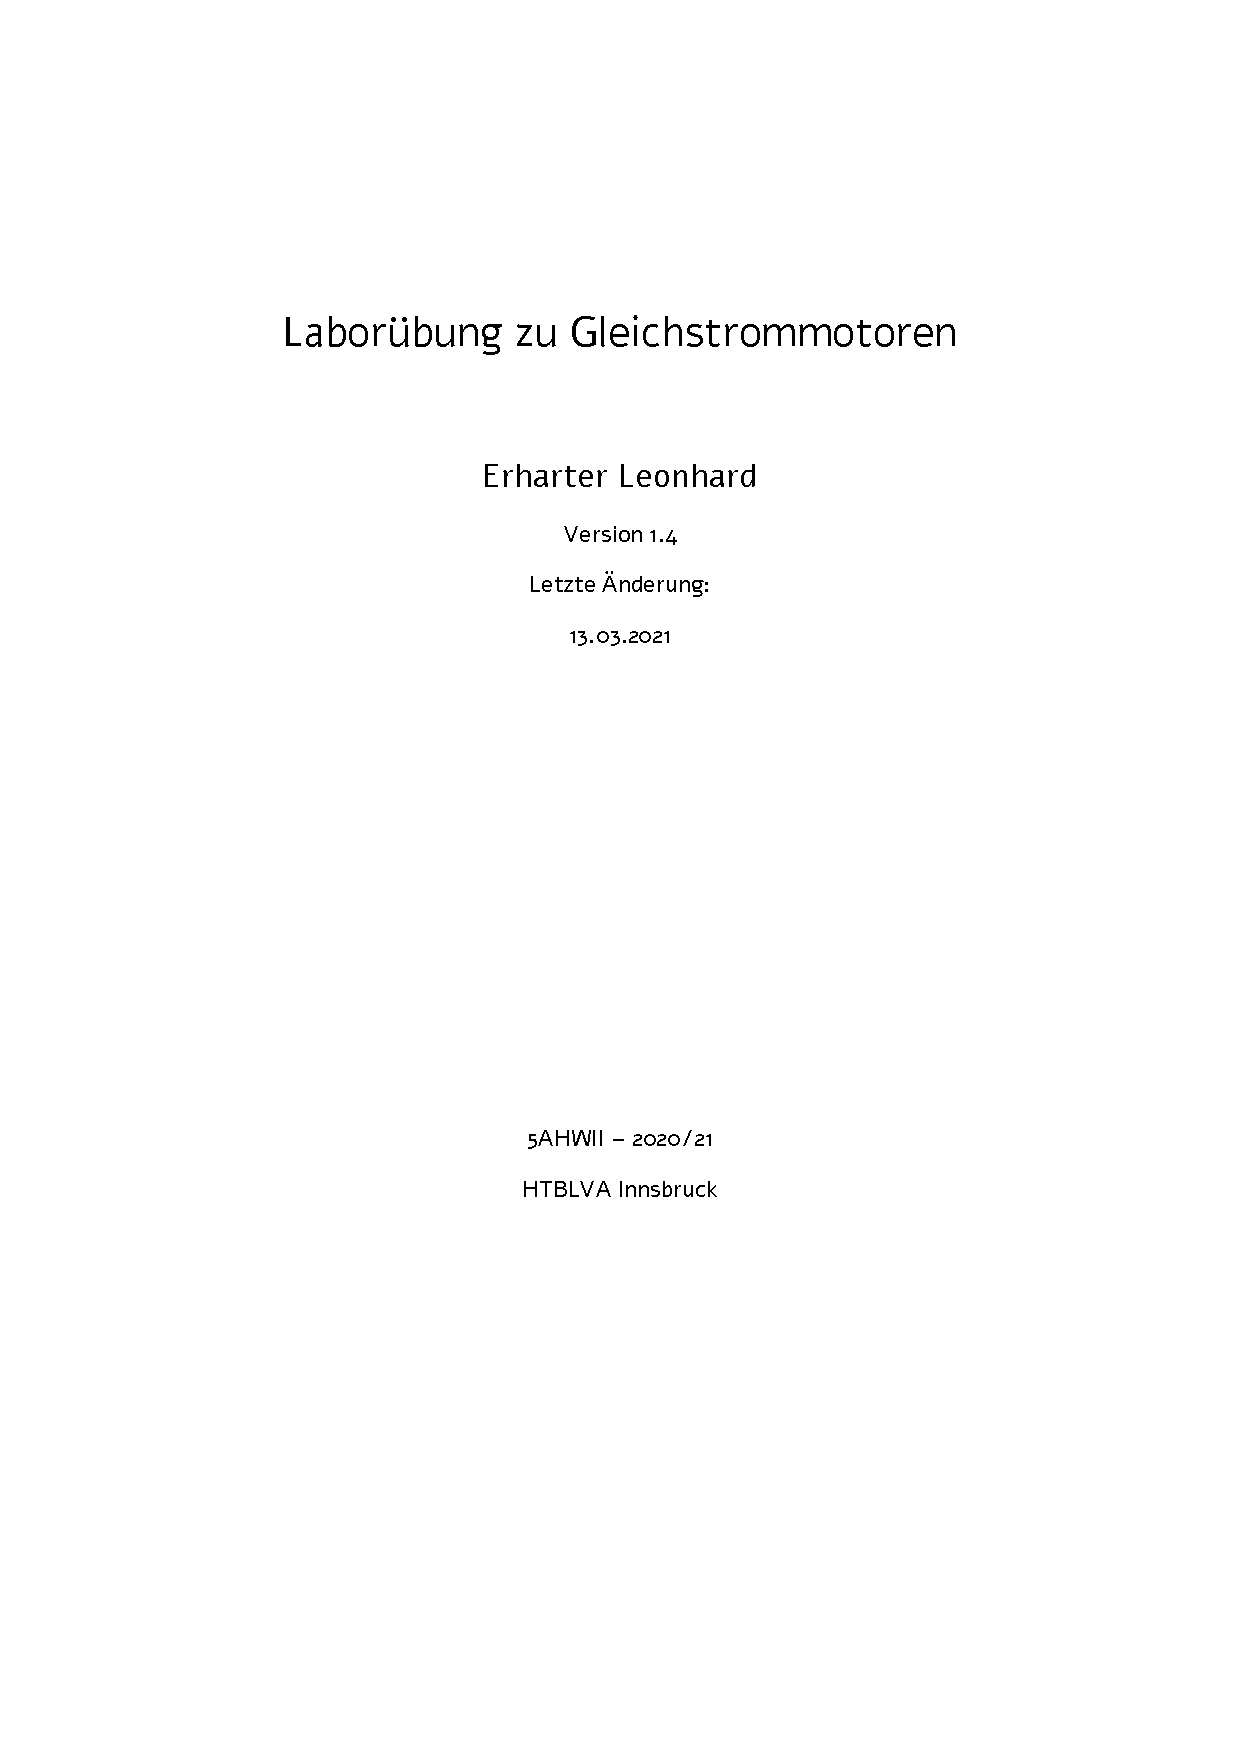
\includepdf[pages=-]{files/LaboruebungV04.pdf}